\newpage

% Chapter 3
 % Write in your own chapter title
\begingroup%
\makeatletter%
\let\clearpage\relax% Stop LaTeX from going to a new page; and
\vspace*{\fill}%
\vspace*{\dimexpr-50\p@-\baselineskip}% Remove the initial (default) 50pt gap (plus 1 line)
\chapterfont{\centering}
\chapter{Proposed Methodology}
\vspace*{\fill}%
\endgroup

\newpage
\label{Chapter3}
\lhead{Chapter 3. \emph{Proposed Methodology}} % Write in your own chapter title to set the page header

\section{General Flow}
The web application we developed offers a wide range of key functionalities and is
easy to use. Our application is designed primarily for administrators and online
users having VR headsets and those who don't have VR headsets as well. The admin can add new products, delete products, update deleted products, view reports/statistics, customer lists, and pending and completed orders. The admin can also update his account setting if necessary. While on the other hand, the customer can visit the website with and without a VR headset as well. Those customers having Oculus VR headsets can experience virtual reality-based MetaMart while customers without VR headsets can do a 3D tour of the MetaMart. The customer can also request some products if not available in our store. Following are some of the diagrams that will help you to understand the sequence flow of our application.
\section{Software development methodology}
We are using Agile methodology.
\subsection{Road map}
Our main goal is to revolutionize the idea of E-Commerce business to facilitate the customer with an immersive and modern virtual platform to bridge the gap between the real and virtual shopping experience. So, to accomplish this goal we came after with the following steps:
\begin{enumerate}
    \item 	Exploring related existing past work (if any), wade through the research papers, articles, and generals. Endeavor to perceive the gaps of prior related works.
    \item Defining a working methodology, which software development approach we are going to manipulate throughout the whole development process.
    \item Specifying the functional and non-functional requirements for the targeted vision.
    \item Conducting feasibility study to contemplate all the aspects of the purposed application model to assemble an estimation is respect to accomplishment extent.
    \item Creating a general flow diagram to accentuate the workflow of the proposed application. Then, design several diagrams including a general diagram, data flow diagram (level0 and level1), use case diagram (general and detailed), flow chart, class diagram, entity-relationship diagram, and sequence diagram to clarify every aspect in a detailed way. 
     \item Note down all the use cases for the MetaMart application.
    \item Afterwards, select the tools and technology going to operate throughout the entire proposal implementation.
    \item Designing the wireframes for web configuration of the virtual environment.
    \item Designing a virtual 3D virtual store in meta verse , 3D clothes, 3D avatars.
    \item Designing the prototype to delineate an explicit scheme of how the proposed application is going to operate.
    \item Finally, developing the MetaMart website and integrating it with the 3D virtual environment made with Unity framework to make the complete system in a fine useable form.
    \item Testing the entire developed system and performing the test case scenarios and evaluating the project according to the test case scenarios.
\end{enumerate}
Feasibility Study:
i)	Economic feasibility:
1.  Web development: almost cost none.
2.  API: some APIs require purchase, so it will account for cost.
3.  Hardware: Our project requires some hardware devices (VR Headsets) which add to the cost of our project. So, to fulfill our economical requirements, we have applied for funding assistance on Ignite FYP funding assistance through the NGIRI portal.

\subsection{Technical feasibility}
The 3D virtual tour and 3D virtual store experience with a VR headset are achievable. With the help of currently available tools to us, it's difficult to make avatars with customized customer input sizes. Regular MetaMart with advanced features like advanced searching filtering, easy navigation, and social media sharing button integration can be done.

\subsection{Operational feasibility}
we will analyze whether our project will work accordingly in the same way as decided. we will also check whether all the features are implemented in the project. So, all the requirements will be fulfilled. we will also keep in the view that our website will be easy to use for customers and should be understandable.

\subsection{	Schedule feasibility}
As for the development process, we will follow the agile methodology in which we will design weekly sprints and in each scheduled meeting, we will improve our system timely. So in his way, the proper schedule will be followed and our product will be completed by the end within the due timeline.

\section{General Proposed Model}
\begin{figure}[H]
    \centering
    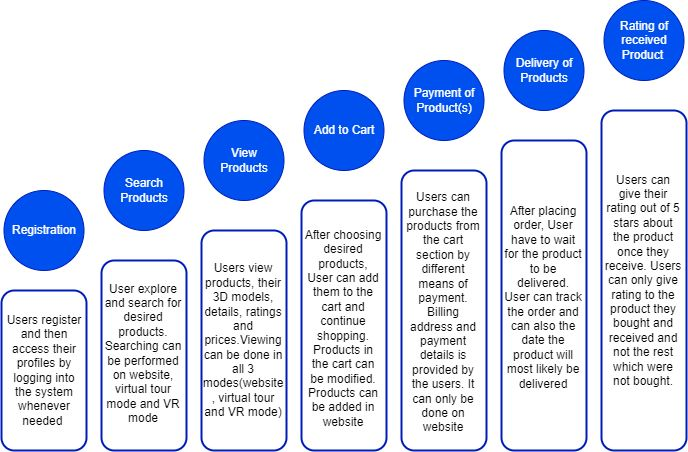
\includegraphics[width=15cm,height=10cm]{Figures/Diagrams/GeneralProposedModel.jpeg}
    \caption{General Proposed Model
     of Virtual Reality-based MetaMart Web Application
     }
    \label{fig: General Proposed Model}
   General Proposed Model
     of Virtual Reality-based MetaMart Web Applications.
\end{figure}
\section{Data Flow Diagram}
Following are the data flow diagrams of the Virtual reality-based MetaMart web application:
\subsection{Data Flow Diagram Level0}
\begin{figure}[H]
    \centering
    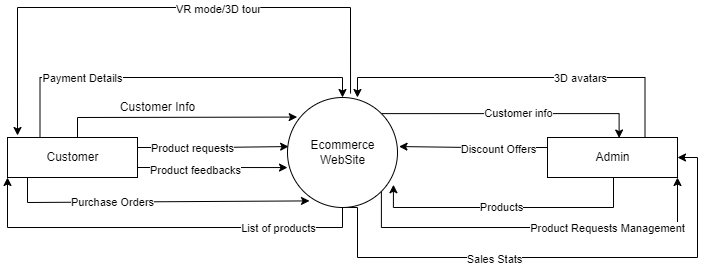
\includegraphics[width=15cm,height=8cm]{Diagrams/dfdlevel0.png}
    \caption{System’s Data Flow Diagram (Level-0)}
    \label{fig: System’s Data Flow Diagram (Level-0)}
\end{figure}
 \justifying
    This diagram illustrates the flow of data between 3 major components of the system which are the customer, admin, and web application. This figure describes which data would be flowing from which source to which destination. As some data like customer information would be flowing from customers towards the application. Similarly, product data would be entered by the admin so this data would be flowing from the admin toward the application. 
\subsection{Data Flow Diagram Level1}
\begin{figure}[H]
    \centering
    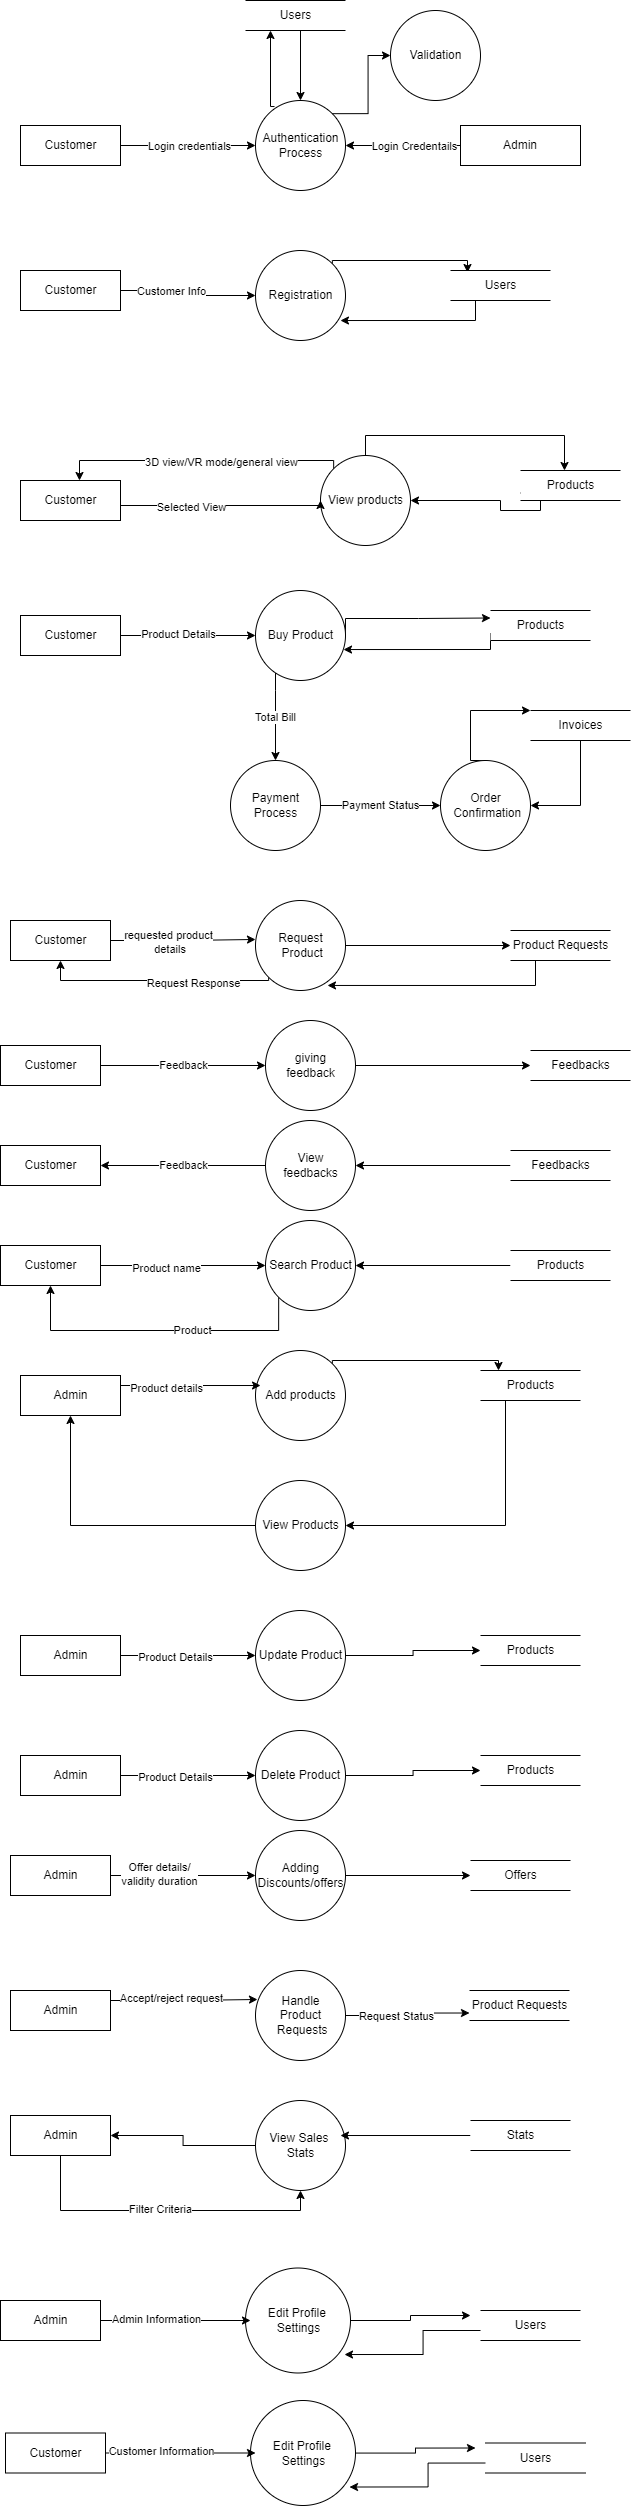
\includegraphics[width=12cm,height=25cm]{Diagrams/dfdlevel1.png}
    \caption{System’s Data Flow Diagram (Level-1)}
    \label{fig: System’s Data Flow Diagram (Level-1)}
\end{figure}
 \justifying
    This diagram illustrates the flow of data between the system’s components by reducing the abstraction level. In this diagram application component in the level-0 diagram is divided into some important modules like giving feedback, making an order, making payment, updating customers’ information, handling request, and many others shown in the diagram. All these modules represent the direction of data, the data which a module consumes or sends to any other dependent module or database.
\section{Use Case Diagram}
In the below section, you will see the General use case diagram and detailed use case diagram of the website as well that describe the high-level functions and scope of a system. 
\subsection{General Diagram}
\begin{figure}[H]
    \centering
    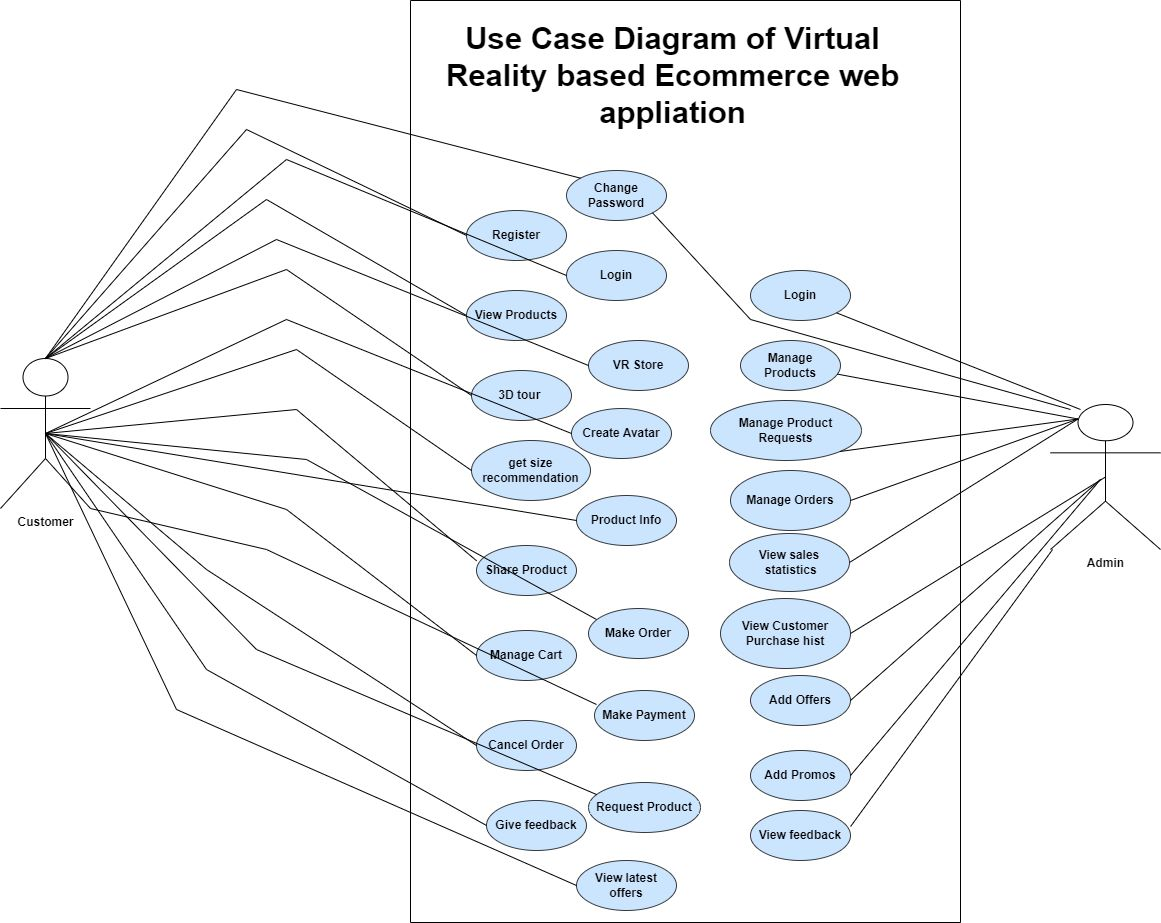
\includegraphics[width=15cm,height=15cm]{Diagrams/GeneralUseCaseDiagram.jpeg}
    \caption{General class Diagram}
    \label{fig: General Use case diagram}
   \justifying
   This diagram represents the general use cases with higher abstraction levels. All the use cases of entities(customer and admin represented by avatars in the diagram) are listed by associating them with the respective entity’s avatar. For example, login is a use case so this use case is associated with the admin’s as well as the customer’s avatar.
\end{figure}
\subsection{Detailed Use case diagram}
\begin{figure}[H]
    \centering
    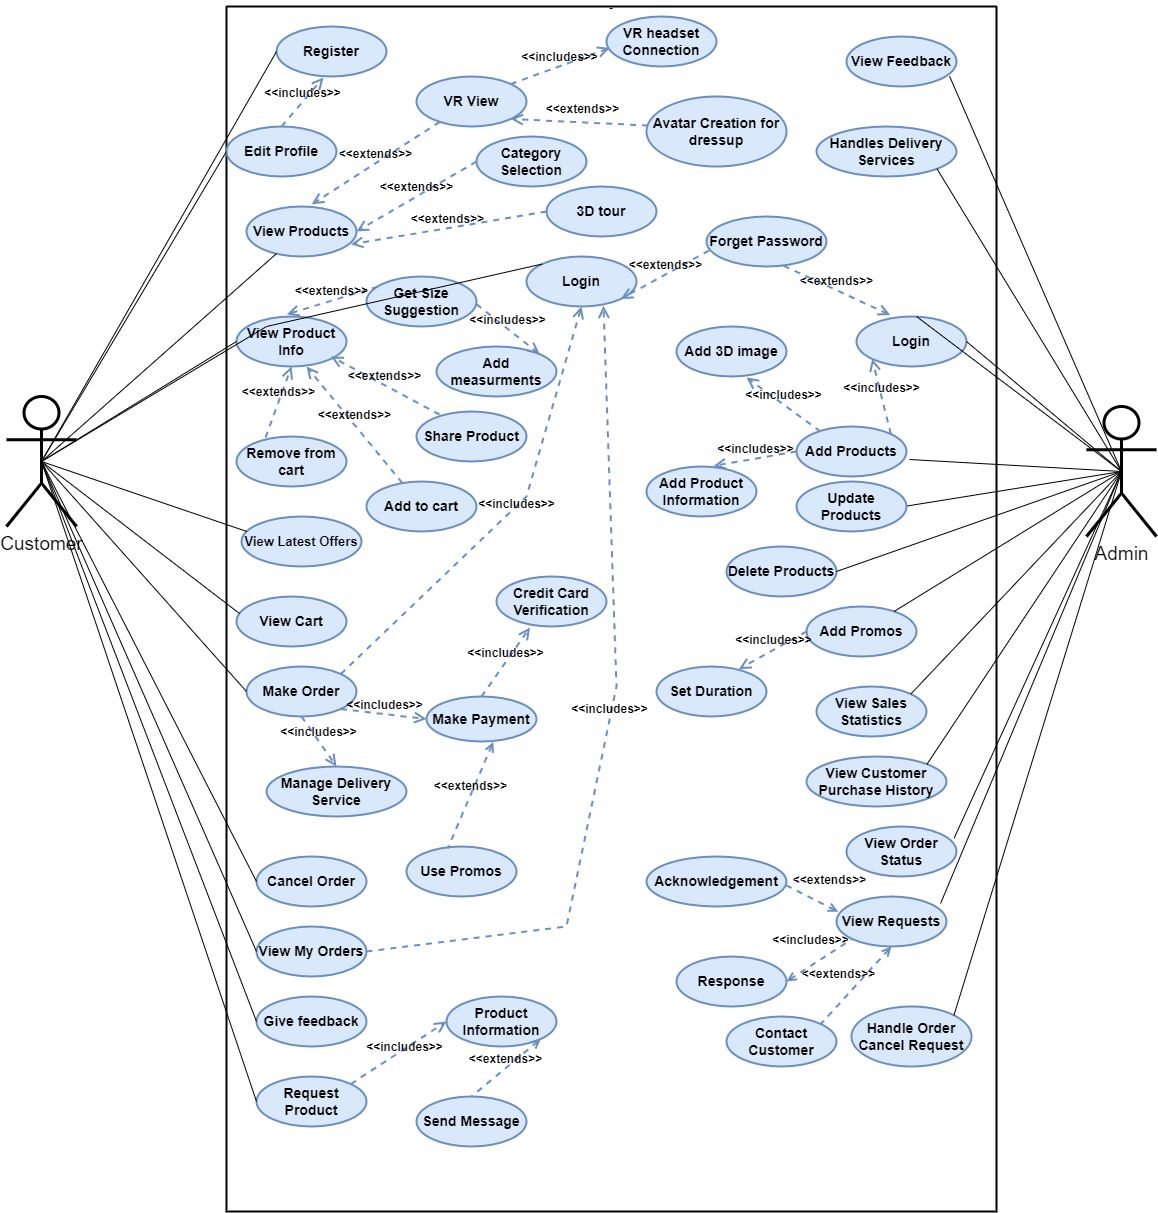
\includegraphics[width=15cm,height=15cm]{Diagrams/DetailUsedCaseDiagram.jpeg}
    \caption{Detailed Use case diagram}
    \label{fig: Detailed Use case diagram}
\end{figure}
\justifying
This diagram represents the detailed use cases. All the use cases of entities are listed along with the relationship(extend/includes) between use cases. For example, login is a use case but another use case which is forgetting the password extends this use case. Similarly, making an order includes making a payment because to complete the first use case (make order),  it is necessary to fulfill included use case which makes payment.
\section{Use Cases}
Following are the actors in our virtual Reality-based MetaMart web application:
\begin{enumerate}
    \item Admin
    \item Customer
\end{enumerate}
\subsection{Use Case of Admin Section}
\subsubsection{Use Case UC-1: Admin Login }
\textbf{Description:}\\
The following use case is about successful administrator login after providing valid login details.
\\
\textbf{Pre-Conditions:}
\begin{enumerate}
    \item Admin should have already been registered.
    \item  All required information about the admin should be available in the database.
    \item Databases should be available.
\end{enumerate}
\textbf{Normal Flow:}\\
\begin{enumerate}
\item The administrator enters valid login details.
\item Administrator clicks on the login button.
\item System confirms and validates the data. 
\item Admin successfully logins the account.
\end{enumerate}
\textbf{Post-Conditions: }
\begin{enumerate}
\item	Admin successfully logins the account. 
\end{enumerate}
\textbf{Authority:}
Administrator
\subsubsection{Use Case UC-2: Add Products }
\textbf{Description:}\\
The following use case is about managing and adding products to the existing system.
\\
\textbf{Pre-Conditions:}
\begin{enumerate}
    \item  All required information about the admin should be available.
    \item Databases should be available.
\end{enumerate}
\textbf{Normal Flow:}\\
\begin{enumerate}
\item Administrator has the option to add a new product.
\item System asks for necessary information regarding the product.
\item Administrator provides all the required information to complete the operation.
\item System after confirmation adds the new product.
\end{enumerate}
\textbf{Post-Conditions: }
\begin{enumerate}
\item	A new user account is successfully created.
\end{enumerate}
\textbf{Authority:}
Administrator
\subsubsection{ Use Case UC-3: Edit Product Details}
\textbf{Description:}\\
The following use case is about managing editing/modifying Product details in the existing system.
\\
\textbf{Pre-Conditions:}
\begin{enumerate}
    \item  All required information about the admin should be available.
    \item Databases should be available.
\end{enumerate}
\textbf{Normal Flow:}\\
\begin{enumerate}
\item Administrator options to edit the product details(title, description, images, etc).
\item Administrator changes the desired details of the product options to complete the operation.
\item System after confirmation updates the details of the product in the database and the website as well.
\end{enumerate}
\textbf{Post-Conditions: }
\begin{enumerate}
\item	The product will be live on the website with updated new details successfully.
\end{enumerate}
\textbf{Authority:}
Administrator
\subsubsection{ Use Case UC-4: Delete Products}
\textbf{Description:}\\
The following use case is about managing to delete products in the existing system.\\
\textbf{Pre-Conditions:}
\begin{enumerate}
    \item  All required information about the admin should be available.
    \item Databases should be available.
\end{enumerate}
\textbf{Normal Flow:}\\
\begin{enumerate}
\item Administrator options to delete a product.
\item The administrator will click on the delete product option and then the system will ask for confirmation before deleting the product from the database.
\item System after confirmation deletes the product from the database.
\end{enumerate}
\textbf{Post-Conditions: }
\begin{enumerate}
\item	The desired product is successfully deleted from the database.
\end{enumerate}
\textbf{Authority:}
Administrator
\subsubsection{ Use Case UC-5: View Products}
\textbf{Description:}\\
The following use case is about viewing products in the existing system.
\\
\textbf{Pre-Conditions:}
\begin{enumerate}
    \item Admin must be logged in to the system.
    \item  All required information about the admin should be available.
    \item Database should be available.
\end{enumerate}
\textbf{Normal Flow:}\\
\begin{enumerate}
\item Administrator options to view a new product.
\item Administrator can see all the products.
\end{enumerate}
\textbf{Post-Conditions: }
\begin{enumerate}
\item	All the products will be displayed to the administrator.
\end{enumerate}
\textbf{Authority:}
Administrator
\subsubsection{ Use Case UC-6: Search Products}
\textbf{Description:}\\
The following use case is about searching for products in the existing system.\\
\textbf{Pre-Conditions:}
\begin{enumerate}
    \item  All required information about the admin should be available.
    \item Database should be available.
\end{enumerate}
\textbf{Normal Flow:}\\
\begin{enumerate}
\item Administrator options to search a product.
\item System asks for necessary information.
\item Administrator provides the name of the product or sets the price range.
\item System after taking administrator shows the results.
\end{enumerate}
\textbf{Post-Conditions: }
\begin{enumerate}
\item	The desired products will be displayed to the admin
\end{enumerate}
\textbf{Authority:}
Administrator
\subsubsection{ Use Case UC-7: View Orders and purchase history of Products}
\textbf{Description:}\\
The following use case is about viewing orders and the purchase history of products in the existing system.
\\
\textbf{Pre-Conditions:}
\begin{enumerate}
    \item  All required information about the admin should be available.
    \item Database should be available.
\end{enumerate}
\textbf{Normal Flow:}\\
\begin{enumerate}
\item Administrator options to about viewing orders and purchase history of products in the existing system.
\item The system will display the orders and purchase history.
\end{enumerate}
\textbf{Post-Conditions: }
\begin{enumerate}
\item	The orders and purchase history of products will be displayed to the admin\end{enumerate}
\textbf{Authority:}
Administrator

\subsubsection{ Use Case UC-8: View Customer Details except for Personal information (account password, credit card password, etc)}
\textbf{Description:}\\
The following use case is about viewing customers in the existing system.
\\
\textbf{Pre-Conditions:}
\begin{enumerate}
\item  Information about the signed-up customers should be available in the existing system.    
\item Database should be available.
\end{enumerate}
\textbf{Normal Flow:}\\
\begin{enumerate}
\item Administrator options about viewing customer details in the existing system.
\item The system will display the customer details(name, total purchasing amount, etc).
\end{enumerate}
\textbf{Post-Conditions: }
\begin{enumerate}
\item	The customer details(name,total purchasing amount etc) will be displayed to the admin
\end{enumerate}
\textbf{Authority:}
Administrator
\subsubsection{ Use Case UC-9: Set discounts and special offers}
\textbf{Description:}\\
The following use case is about setting the discount price on the products.
\\
\textbf{Pre-Conditions:}
\begin{enumerate}
    \item  All required information about the admin should be available.
    \item Database should be available.
\end{enumerate}
\textbf{Normal Flow:}\\
\begin{enumerate}
\item While adding a new product the admin can set the discount on the product or the option will be provided to the admin from which the admin can set the discount prices on the products based on the price range etc.
\end{enumerate}
\textbf{Post-Conditions: }
\begin{enumerate}
\item	The product with a discount price will be shown to the customer will be displayed to the admin
\end{enumerate}
\textbf{Authority:}
Administrator
\subsubsection{ Use Case UC-10: Administrator Logout}
\textbf{Description:}\\
The following use case is about successfully logging out administrators.
\\
\textbf{Pre-Conditions:}
\begin{enumerate}
    \item Admin must be logged in through valid login details.
    \item  Admin must be able to perform all the required operations.
    \item  There must be an option to log out as an administrator.
    \item Databases should be available.
\end{enumerate}
\textbf{Normal Flow:}\\
\begin{enumerate}
\item Administrator logins the account.
\item System validates the data. 
\item Administrator successfully logs into the account. 
\item Administrator performs all the required operations.
\item Administrator clicks on the logout button. 
\item System successfully logs out the administrator.
\end{enumerate}
\textbf{Alternative flow:} \\ 
2a. There is a problem with the Admin login account. 
 \\
\begin{itemize}
    \item Admin can recover password using forgot password.
     \item Admin can again try to login Admin continues from step 1.
\end{itemize}
\textbf{Post-Conditions: }
\begin{enumerate}
\item	The administrator successfully logs out of the system.
\end{enumerate}
\textbf{Authority:}
Administrator

\subsection{Use Case of Customer Section}
        
\subsubsection{Use Case UC-1: User Sign Up}
\textbf{Description:}\\
The following use case is about adding a new user to an existing system. A new user can sign up any time he wants if he hasn’t already made an account. 
\\
\textbf{Pre-Conditions:}
\begin{enumerate}
    \item  All required information about the admin should be available.
    \item Databases should be available.
\end{enumerate}
\textbf{Normal Flow:}\\
\begin{enumerate}
\item  New User by clicking on the signup button opts for creating a new account.
\item  System asks for necessary information. 
\item  User provides all the required information and opts to complete the operation.
\item  System confirms and validates the data. 
\item  System creates a new account successfully. 
\item  System sends the account creation email to the administrator’s email id and user’s email
\end{enumerate}
Alternative flow: \\
1a. There is a problem with the User’s login details. Required information is not provided.
\begin{itemize}
    \item 	Users can check the login details and correct them.
     \item The user continues from step 1. 
\end{itemize}
3a. There is a problem with the data provided, some data needs to be corrected.
\begin{itemize}
    \item The user checks the available information and corrects the error. 
     \item The user continues from step 3. 
\end{itemize}	
	4a. There is a problem with the data validation. The data provided is not valid.  
	 \begin{itemize}
    \item 	The user checks the validation of data and corrects the information.
     \item 	The user continues from step 3. 
\end{itemize}	

\textbf{Post-Conditions: }
\begin{enumerate}
\item	A new User account was successfully created.
\item	New Users can log in to the account using his/her login details.
\end{enumerate}
\textbf{Authority:}
User
\subsubsection{Use Case UC-2: User Login}
\textbf{Description:}\\
The following use case is about successful User login after providing valid login details. 
\\
\textbf{Pre-Conditions:}
\begin{enumerate}
    \item Users should have already been registered.
    \item  All required information about the admin should be available in the database.
    \item Databases should be available.
\end{enumerate}
\textbf{Normal Flow:}\\
\begin{enumerate}
\item User enters valid login details. 
\item User clicks on the login button. 
\item System confirms and validates the data. The user successfully logs in to the account.
\end{enumerate}
Alternative flow: \\
1a. There is a problem with the User’s login details.
\begin{itemize}
    \item The user provides the required login details. 
    \item 	The User continues from step 1.
\end{itemize}
3a. There is a problem with the data provided, some data needs to be corrected.
\begin{itemize}
    \item The user checks the available information and corrects the error. 
    \item 	The user continues from step 3. 
\end{itemize}
3b. There is a problem with the data validation. The data provided is not valid. 
\begin{itemize}
    \item The user checks the validation of data and corrects the information. 
    \item User recovers password if forgotten using forgot password link. 
    \item The user continues from step 3.
\end{itemize}
\textbf{Post-Conditions: }
\begin{enumerate}
\item	The user successfully logs in to the account. 
Open Issues: if the database fails to connect, the user may need to wait for days to connect.
\end{enumerate}
\textbf{Authority:}
User
\subsubsection{Use Case UC-3: User Profile Creation }
\textbf{Description:}\\
The following use case is about the successful creation of a user profile after providing valid profile details. 
\\
\textbf{Pre-Conditions:}
\begin{enumerate}
    \item Users should have already been registered.
    \item  All required information about the admin should be available in the database.
    \item Databases should be available.
\end{enumerate}
\textbf{Normal Flow:}\\
\begin{enumerate}
\item User enters valid required details for creating a profile. 
\item User clicks on the create profile button. 
\item System confirms and validates the data.
\item User successfully creates a profile.
 \end{enumerate}
\textbf{Alternative flow:}  \\
1a. There is a problem with the User’s profile details. 
\begin{itemize}
    \item 	The user provides the required details when creating a profile. 
    \item  The user continues from step 1.
\end{itemize}
3a. There is a problem with the data provided, some data needs to be corrected. 
\begin{itemize}
    \item 	The user checks the available information and corrects the error. 
     \item 	The user continues from step 3. 
\end{itemize}
3b. There is a problem with the data validation. The data provided is not valid.
\begin{itemize}
    \item The user checks the validation of data and corrects the information. 
     \item The user continues from step 3
\end{itemize}	
\textbf{Post-Conditions: }
\begin{enumerate}
\item	The user successfully creates a profile. 
Open Issues: if the database fails to connect, the user may need to wait for days to connect.
\end{enumerate}
\textbf{Authority:}
User
\subsubsection{Use Case UC-4: Edit Account Information}
\textbf{Description:}\\
The following use case is about the user changing their account details successfully. 
\\
\textbf{Pre-Conditions:}
\begin{enumerate}
    \item Users should be already logged in.
    \item  All required information about the admin should be available in the database.
    \item Databases should be available.
\end{enumerate}
\textbf{Normal Flow:}\\
\begin{enumerate}
\item User navigates to the account setting page. 
\item User edits its details and saves. 
\item For confirmation, the user is asked to write the password twice.
\item System confirms and validates the data.
\item User account is successfully updated. 
\end{enumerate}
\textbf{Alternative flow:}\\ 
2a. There is a problem with the User’s profile details.
\begin{itemize}
    \item The user will be provided with validation in case they enter invalid data such as number in name etc. 
    \item The user continues from step 2.
\end{itemize}
3a. There is a problem with the data provided, some data needs to be corrected. 
\begin{itemize}
    \item If the user enters the wrong password, then they will be asked to provide the correct password to continue to update details. 
    \item The user continues from step 3.
\end{itemize}
\textbf{Post-Conditions: }
\begin{enumerate}
\item	The user successfully updates their profile details.
\end{enumerate}
\textbf{Authority:}
User
\subsubsection{Use Case UC-5: Switching to Virtual tour mode }
\textbf{Description:}\\
The following use case is about users switching to virtual tour mode on the website for a better experience of products and a realistic feel. 
\\
\textbf{Pre-Conditions:}
\begin{enumerate}
 \item Users should be logged in. 
\item Option will be available on the website for virtual tour mode.
\item User will have to select his desired avatar from the available ones.
\item Proper description and measurement of avatar will be provided. 
\item Databases should be available. 
\end{enumerate}
\textbf{Normal Flow:}\\
\begin{enumerate}
\item User clicks the virtual tour option and switches to virtual tour mode for a better experience. 
\item User controls the avatar and roams around the virtual store and views products. 
\item After viewing user can also add the item to the cart in the same mode. 
\end{enumerate}
\textbf{Alternative flow:}\\ 
2a. In case the user has not selected his/her avatar previously
\begin{itemize}
    \item The user will first be provided with the list of avatars and their measurement details.
     \item The user selects the avatar according to his/her preference.
     \item The user continues from step 2. 
 \end{itemize}
\textbf{Post-Conditions: }
\begin{enumerate}
\item	The user successfully explores the virtual tour mode.
\item	The option will be available which can navigate the user back to the website
\end{enumerate}
\textbf{Authority:}
User
\subsubsection{Use Case UC-6: Switching to VR mode}
\textbf{Description:}\\
The following use case is about users switching to VR mode from the website for a better experience of products and a realistic feel. 
\\
\textbf{Pre-Conditions:}
\begin{enumerate}
 \item Users should be logged in. 
\item Users should have VR headsets compatible with the system.
\item Option will be available on the website for switching to VR mode.
\item User will have to select his desired avatar from the available ones.
\item Proper description and measurement of avatar will be provided. 
\item Databases should be available.\end{enumerate}
\textbf{Normal Flow:}\\
\begin{enumerate}
\item The user clicks the VR mode option on the website.
\item The user configures a VR headset (such as Oculus) with the system
\item After configuration, the user is connected to his/her selected avatar and can roam around the virtual store and view products. 
\item After viewing user can also add the item to the cart in the same mode. 
\end{enumerate}
\textbf{Alternative flow:}\\  
2a. In case the user’s VR headset is not compatible
\begin{itemize}
    \item Users cannot experience VR mode and have to continue to the website or virtual tour mode.
\end{itemize}
3a. In case the user has not selected his/her avatar previously.
\begin{itemize}
    \item The user will first be provided with the list of avatars and their measurement details.
    \item The user selects the avatar according to his/her preference.
    \item	The user continues from step 3.
\end{itemize}
\textbf{Post-Conditions: }
\begin{enumerate}
\item	The user successfully explores the VR mode.
\item	The option will be available which can navigate the user back to the website and the VR headset will be disconnected from the system. 
\end{enumerate}
\textbf{Authority:}
User
\subsubsection{Use Case UC-7: Add to Cart (Website)}
\textbf{Description:}\\
The following use case is about adding products to the cart so that users could checkout.
\\
\textbf{Pre-Conditions:}
\begin{enumerate}
    \item User may or may not be logged in for an add-to-cart operation.
 \item Similar items can be added more than one time. 
 \item Number will be shown on the cart icon displaying the number of products in the cart.
 \item Add to cart button will only be shown on in-stock available products.
 \item Databases should be available.\end{enumerate}
\textbf{Normal Flow:}\\
\begin{enumerate}
\item User picks a product and presses add to cart button. 
\item Users can search for more products and add those as well. 
\item User clicks on the cart icon to navigate to the cart page. 
\item User validates the selected products and proceeds to the checkout page. 
\item If the user is not satisfied, products added to the cart can be removed and the user can get navigated back to the products page. 
\end{enumerate}
\textbf{Alternative flow:}\\ 
1a. In case the user picks a product but it is not available in stock. 
\begin{itemize}
    \item Add to cart button won't be clickable.  
  \item   User continues from step 1 for different(available) products.
\end{itemize}	
4a. In case the user is not logged in.
\begin{itemize}
    \item 	After clicking the checkout button, the user will first be directed to the login page and asked for credentials
    \item After successful login, the user will be redirected back to the checkout page.
    \item The user proceeds to checkout.
\end{itemize}	
\textbf{Post-Conditions: }
\begin{enumerate}
\item	The user successfully adds products to the cart.
\end{enumerate}
\textbf{Authority:}
User

\subsubsection{Use Case UC-8: Add to Cart (Virtual Tour mode) }
\textbf{Description:}\\
The following use case is about adding products to the cart in Virtual tour mode so that users could checkout. \\
\textbf{Pre-Conditions:}
\begin{enumerate}
    \item The user must be logged in for an add-to-cart operation in virtual tour mode.
\item The user will be in virtual tour mode.
 \item Similar items can be added more than one time. 
 \item Number will be shown on the cart icon displaying the number of products in the cart.
 \item Add to cart button will only be shown on in-stock available products
 \item Databases should be available. 
\end{enumerate}
\textbf{Normal Flow:}\\
\begin{enumerate}
\item User picks a product and presses add to cart button. 
\item Users can search for more products by roaming around the virtual store. 
\item User clicks on the cart icon to navigate to the cart page. 
\item User validates the selected products and proceeds to the checkout page. 
\item If the user is not satisfied, products added to the cart can be removed and the user can get navigated back to virtual tour mode. 
\end{enumerate}
\textbf{Alternative flow:}

1a. In case the user picks a product but it is not available in stock. 
\begin{itemize}
    \item 	Add to cart button won't be clickable.
     \item User continues from step 1 for different(available) products.
\end{itemize}
\textbf{Post-Conditions: }
\begin{enumerate}
\item	User successfully adds products to cart in virtual tour mode.
\end{enumerate}
\textbf{Authority:}
User
\subsubsection{Use Case UC-9: Add to Cart (VR mode) }
\textbf{Description:}\\
The following use case is about adding products to the cart in VR mode so that users could checkout. \\
\textbf{Pre-Conditions:}
\begin{enumerate}
    \item The user must be logged in for an add-to-cart operation in VR mode.
\item The user will be in VR mode.
 \item Similar items can be added more than one time. 
 \item Number will be shown on the VR headset screen displaying the number of products in the cart.
 \item Add to cart option will only be shown on in-stock available products
 \item Databases should be available. \end{enumerate}
\textbf{Normal Flow:}\\
\begin{enumerate}
\item User picks a product and moves the hand to the add-to-cart option for adding it to the cart. 
\item Users can search for more products by roaming around the VR mode. 
\item User moves the hand on the cart icon on the headset screen to navigate to the cart page. 
\item User validates the selected products and proceeds to the checkout page. 
\item If the user is not satisfied, products added to the cart can be removed and the user can get back to product view in VR mode. 
\end{enumerate}
\textbf{Post-Conditions: }
\begin{enumerate}
\item	Admin successfully logins the account. 
\end{enumerate}
\textbf{Authority:}
Administrator
\subsubsection{Use Case UC-10: View Products (Website)}
\textbf{Description:}\\
The following use case is about viewing available products on the web page. 
\\
\textbf{Pre-Conditions:}
\begin{enumerate}
    \item User may or may not be logged in for viewing products.
 \item Search and product filtering options will be provided. 
 \item Different sorts of options for products will be available.
 \item Image and proper description with feedback and ratings will be provided when any particular product is selected.
 \item Databases should be available. \end{enumerate}
\textbf{Normal Flow:}\\
\begin{enumerate}
\item With or Without login, the User views the products page. 
\item Users can use the search option and filter for quick desired output. 
\item User clicks the particular product and is directed to a page including all of the details of that product. 
\item User checks all descriptions, feedback, rating, etc of the product and adds it to the cart if satisfied. 
\end{enumerate}
\textbf{Alternative flow:} \\
3a. In case the user does not want to visit the page consisting of that particular product. 
\begin{itemize}
    \item Users can add them to the cart the product without having to see its details.
    \item The user continues from step 1 for more products or visits the cart page.
\end{itemize}
4a. In case the user is not satisfied fully and wants to test the product (wearable item).
\begin{itemize}
    \item Users can go to a 3D environment or VR mode.
    \item There they can test the wearable item with different on its selected custom virtual avatar for fitting issues.
  \item 	After satisfaction, the user can add to the cart that product from the 3D environment/VR mode.
 \item  The user either continues in the same environment for viewing more products or goes back to website mode.
\end{itemize}
\textbf{Post-Conditions: }
\begin{enumerate}
\item	Users can efficiently view products in website mode.
\end{enumerate}
\textbf{Authority:}
User
\subsubsection{Use Case UC-11: View Products (Virtual Tour mode) }
\textbf{Description:}\\
The following use case is about viewing available products in the virtual tour mode. 
\\
\textbf{Pre-Conditions:}
\begin{enumerate}
    \item User must be logged in for viewing products in virtual tour mode.
 \item 3D models Products will be placed in the virtual store already. 
\item Proper description with feedback and ratings will be provided when any particular 3d model of the product is selected.
 \item Databases should be available. 
\end{enumerate}
\textbf{Normal Flow:}\\
\begin{enumerate}
\item The user roams around the store using a selected avatar to see 3D models of products. 
\item User clicks the particular 3D model of details and the description of the product is shown. 
\item For wearable items, the user can virtually try on the item on the avatar and check the fitting of any size by rotating the avatar 
\item User checks all descriptions, feedback, rating, and virtual try-on of the product and adds it to the cart if satisfied. 
\end{enumerate}
\textbf{Post-Conditions: }
\begin{enumerate}
\item	Users can efficiently view products in virtual tour mode.
\end{enumerate}
\textbf{Authority:}
User
\subsubsection{Use Case UC-12: View Products (VR mode) }
\textbf{Description:}\\
The following use case is about viewing available products in VR mode. 
\\
\textbf{Pre-Conditions:}
\begin{enumerate}
    \item User must be logged in for viewing products in VR mode.
\item 3D models Products will be placed in the virtual store already. 
\item Proper description with feedback and ratings will be provided when any particular 3d model of the product is selected.
 \item Databases should be available. 
\end{enumerate}
\textbf{Normal Flow:}\\
\begin{enumerate}
\item The user roams around the store using a VR headset as an avatar to see 3D models of products. 
\item Users can grab the particular 3D model virtually.
\item User hovers over the particular 3D model of details and the description of the product is shown. 
\item For wearable items, the user can virtually try on the item on the avatar and check the fitting of any size by rotating the avatar 
\item User checks all descriptions, feedback, rating, and virtual try-on of the product and adds it to the cart if satisfied. 
\end{enumerate}
\textbf{Post-Conditions: }
\begin{enumerate}
\item	Users can efficiently view products in VR mode.
\end{enumerate}
\textbf{Authority:}
User
\subsubsection{Use Case UC-13: Giving feedback (Website) }
\textbf{Description:}\\
The following use case is about giving feedback on the web page. 
\\
\textbf{Pre-Conditions:}
\begin{enumerate}
    \item The user must be logged in for giving feedback.
\item Previous feedback given by others should be visible to the user.
\item Databases should be available. 
\end{enumerate}
\textbf{Normal Flow:}\\
\begin{enumerate}
\item The user selects any products. 
\item The user writes their feedback on the feedback area about that product or can ask any question regarding it. 
\item The user clicks the submit button to send feedback. 
\item The user waits for a response from the administrator side \end{enumerate}
\textbf{Post-Conditions: }
\begin{enumerate}
\item	Users can efficiently give feedback about products, delivery responses, etc. 
\end{enumerate}
\textbf{Authority:}
User
      
\subsubsection{Use Case UC-14: Giving rating (Website) }
\textbf{Description:}\\
The following use case is about giving a rating on the web page. 
\\
\textbf{Pre-Conditions:}
\begin{enumerate}
    \item The user must be logged in for giving a rating to the product.
\item The current rating of the product and the number of ratings should be visible to the user.
\item Databases should be available. 
\end{enumerate}
\textbf{Normal Flow:}\\
\begin{enumerate}
\item The user selects any products. 
\item The user will be shown five empty stars.
\item The user has to give their rating from one to five stars about that product.
\item User selects the rating and their rating will be added to the product. 
\end{enumerate}
\textbf{Alternative flow: }\\
2a. If the user already gave a rating to the product
\begin{itemize}
    \item User will be shown their previous rating
     \item Users can edit the rating by clicking it and choosing a new rating.
\end{itemize}
\textbf{Post-Conditions: }
\begin{enumerate}
\item	Users can efficiently give a rating to a product.
\end{enumerate}
\textbf{Authority:}
User
   
\subsubsection{Use Case UC-15: Order History of Products }
\textbf{Description:}\\
The following use case is about user viewing their all order history on the web page. 
\\
\textbf{Pre-Conditions:}
\begin{enumerate}
    \item The user must be logged in for viewing their order history.
\item Databases should be available. 
\end{enumerate}
\textbf{Normal Flow:}\\
\begin{enumerate}
\item The user goes to the order history page. 
\item The user sees all details and pricing of all previously completed or uncompleted orders. \end{enumerate}
\textbf{Alternative Flow:}\\
2a. In case the user has not purchased anything previously. 
\begin{itemize}
\item 	An empty message will be displayed stating that No previous completed orders yet
\end{itemize}

\textbf{Post-Conditions: }
\begin{enumerate}
\item Users can efficiently view previous history details.
\end{enumerate}
\textbf{Authority:}
User
\subsubsection{Use Case UC-16: Pending Orders (Website) }
\textbf{Description:}\\
The following use case is about the user viewing all pending (yet to be delivered) order history on the web page.
\\
\textbf{Pre-Conditions:}
\begin{enumerate}
    \item The user must be logged in for viewing pending orders.
\item Databases should be available.
\end{enumerate}
\textbf{Normal Flow:}\\
\begin{enumerate}
\item The user goes to the pending orders. 
\item The user sees all details of the upcoming product(s) to be delivered with the delivery date. \end{enumerate}
\textbf{Alternative Flow:}\\
2a. In case the user has nothing yet to be delivered. \begin{itemize}
    \item An empty message will be displayed stating that nothing is to be delivered yet
\end{itemize}
\textbf{Post-Conditions: }
\begin{enumerate}
\item	Users can efficiently view previous history details.
\end{enumerate}
\textbf{Authority:}
User
 
\subsubsection{Use Case UC-17: User Logout }
\textbf{Description:}\\
The following use case is about successfully logging out users. 
\\
\textbf{Pre-Conditions:}
\begin{enumerate}
    \item Users must be logged in through valid login details.
  \item Users must be able to perform all the required operations. 
  \item There must be an option to log out for Users.
  \item Databases should be available. 
\end{enumerate}
\textbf{Normal Flow:}\\
\begin{enumerate}
\item User logs in to the account. 
\item System validates the data. 
\item Users successfully log in to the account. 
\item Users perform all the required operations. 
\item Users click on the logout button. 
\item System successfully logs out the user. 
\end{enumerate}
\textbf{Alternative flow: }\\
2a. There is a problem with the user’s login account. \begin{itemize}
\item Users can recover passwords using the forgotten password option. 
\item Users can again try to log in. 
\item User continues from step 1

\end{itemize}
\textbf{Post-Conditions: }
\begin{enumerate}
\item	The user successfully logs out of the system.
\end{enumerate}
\textbf{Authority:}
User
\section{Flow Chart}
\begin{figure}[H]
    \centering
    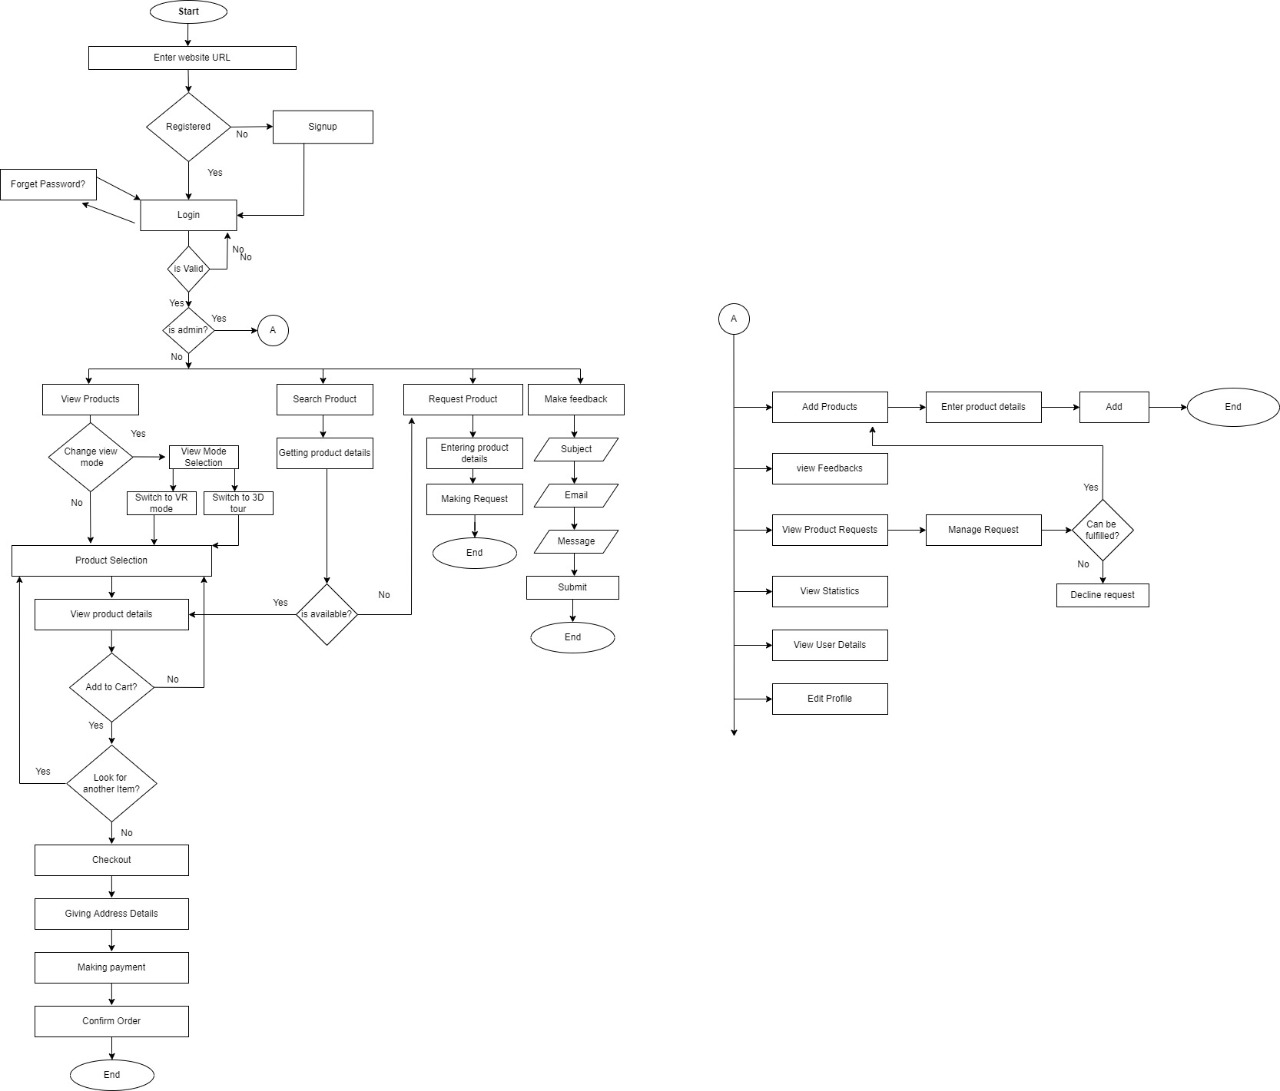
\includegraphics[width=14cm,height=15cm]{Diagrams/FlowChart.jpeg}
    \caption{System’s flowchart diagram}
    \label{fig: System’s flowchart diagram}
    \end{figure}
    \justifying
    This diagram represents the flow of processes. These processes are those which are highly focused during the development of the system. From start to end, the diagram covers all the important steps that are necessary to list there. On the customer side majorly three 3 processes have been listed which are buying a product, requesting a product, and making feedback for the purchased product. Similarly, all processes done by the admin are listed there.

\section{Architectural Diagram}
\subsection{Contextual Diagram}
\begin{figure}[H]
    \centering
    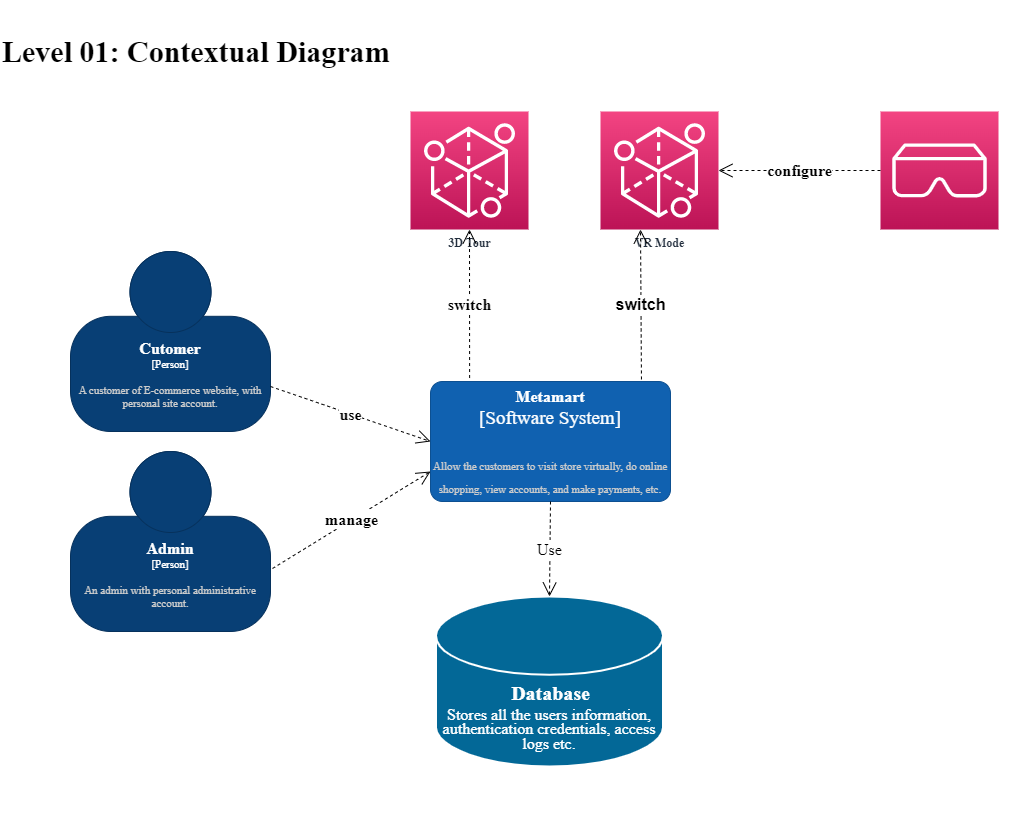
\includegraphics[width=15cm,height=15cm]{Figures/Diagrams/ArchitecturalDiagram/ContextualDiagram.png}
    \caption{Contextual Diagram}
    \label{Contextual Diagram}
\end{figure}
\subsection{Container Diagram}
\begin{figure}[H]
    \centering
    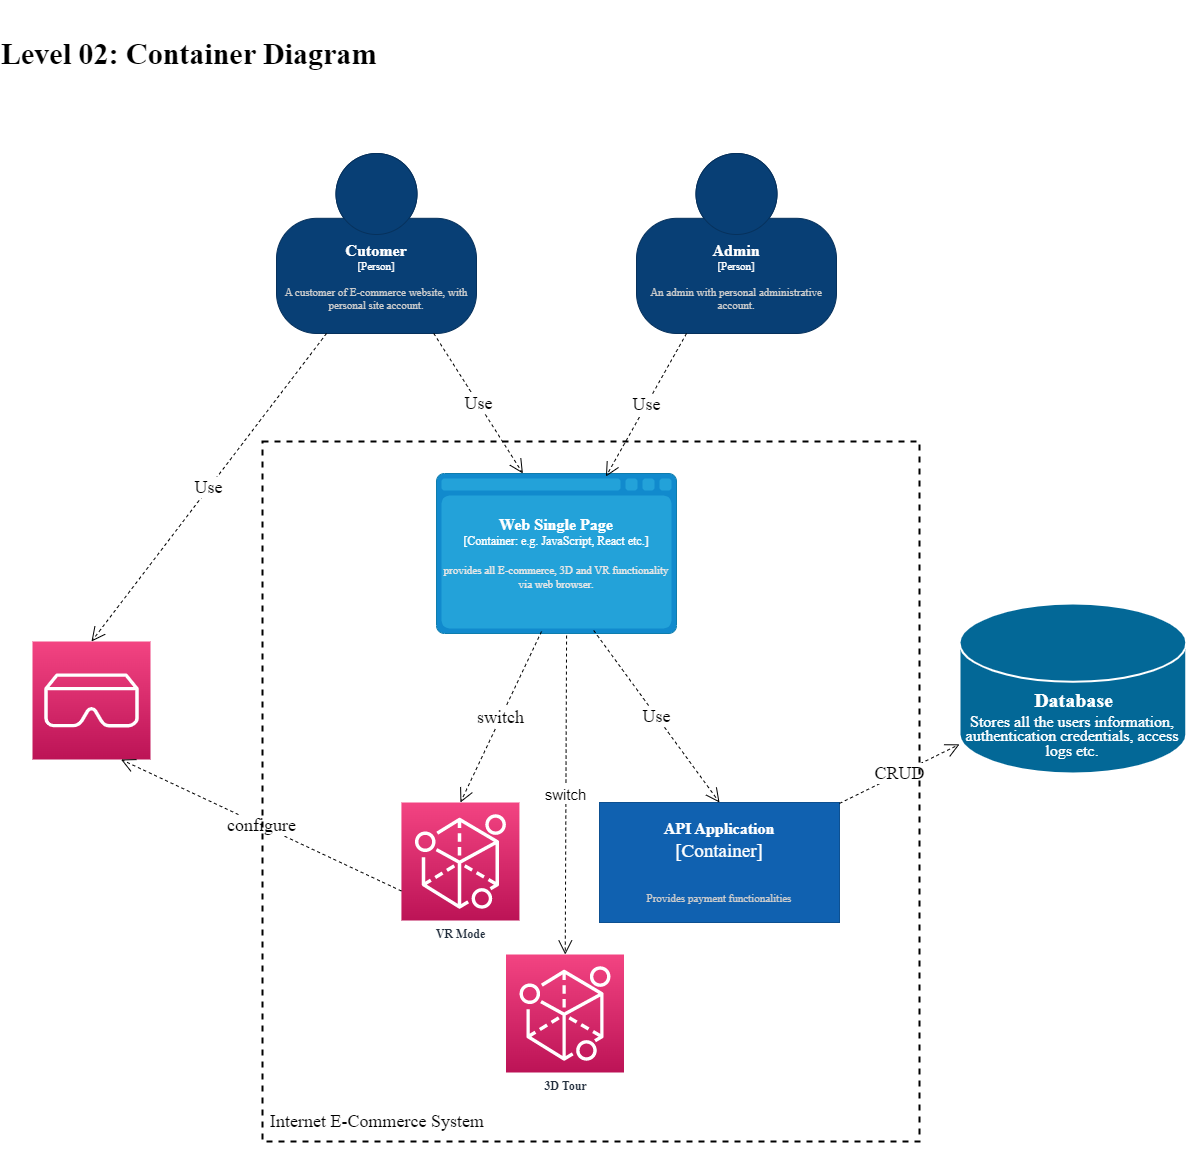
\includegraphics[width=15cm,height=15cm]{Figures/Diagrams/ArchitecturalDiagram/ContainerDiagram.png}
    \caption{Container Diagram}
    \label{Container Diagram}
\end{figure}
\subsection{Component  Diagram}
\begin{figure}[H]
    \centering
    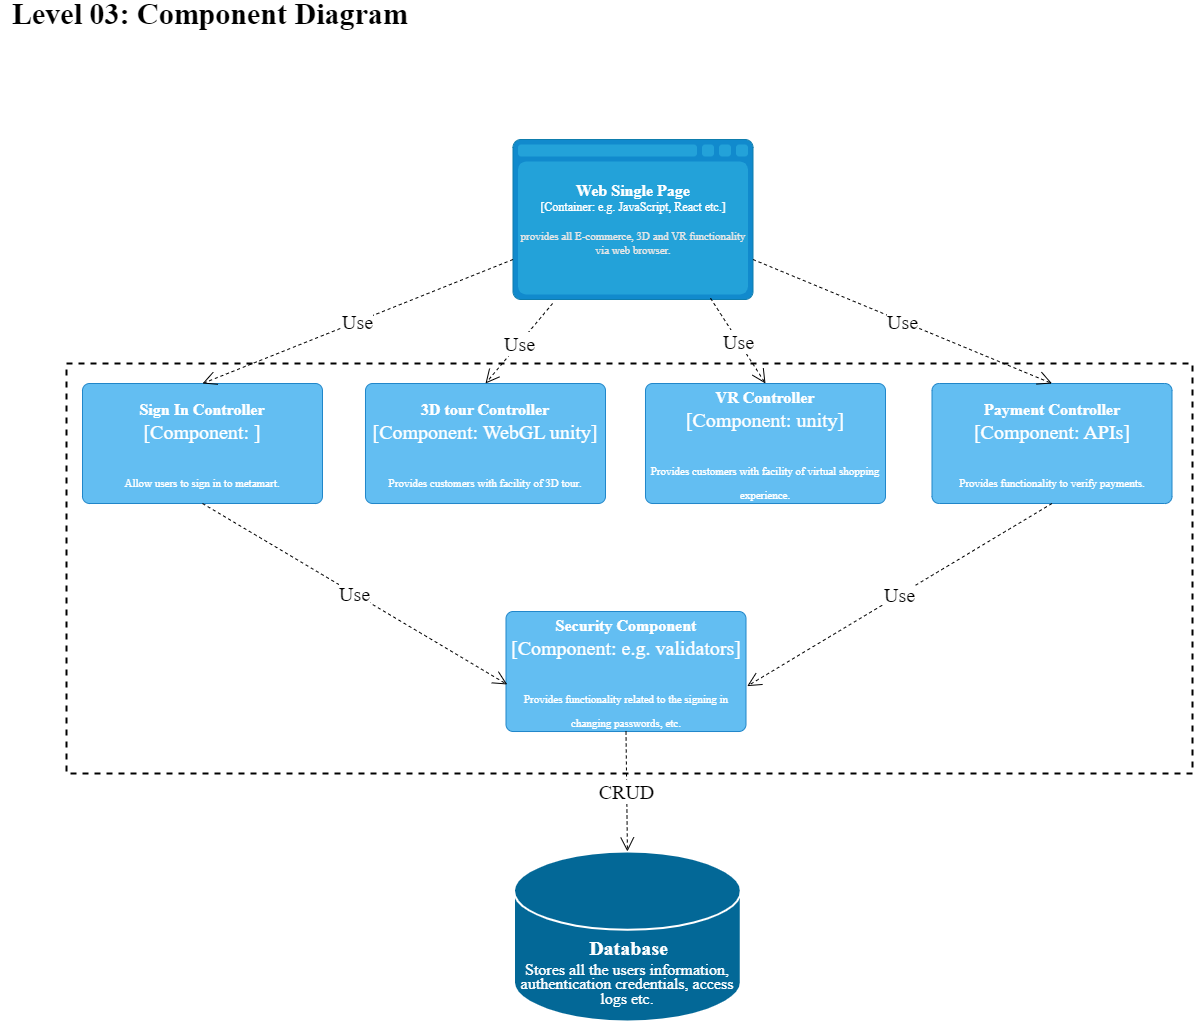
\includegraphics[width=14cm,height=15cm]{Figures/Diagrams/ArchitecturalDiagram/ComponentDiagram.png}
    \caption{Component Diagram}
    \label{Component Diagram}
\end{figure}
\section{Class Diagram}
\begin{figure}[H]
    \centering
    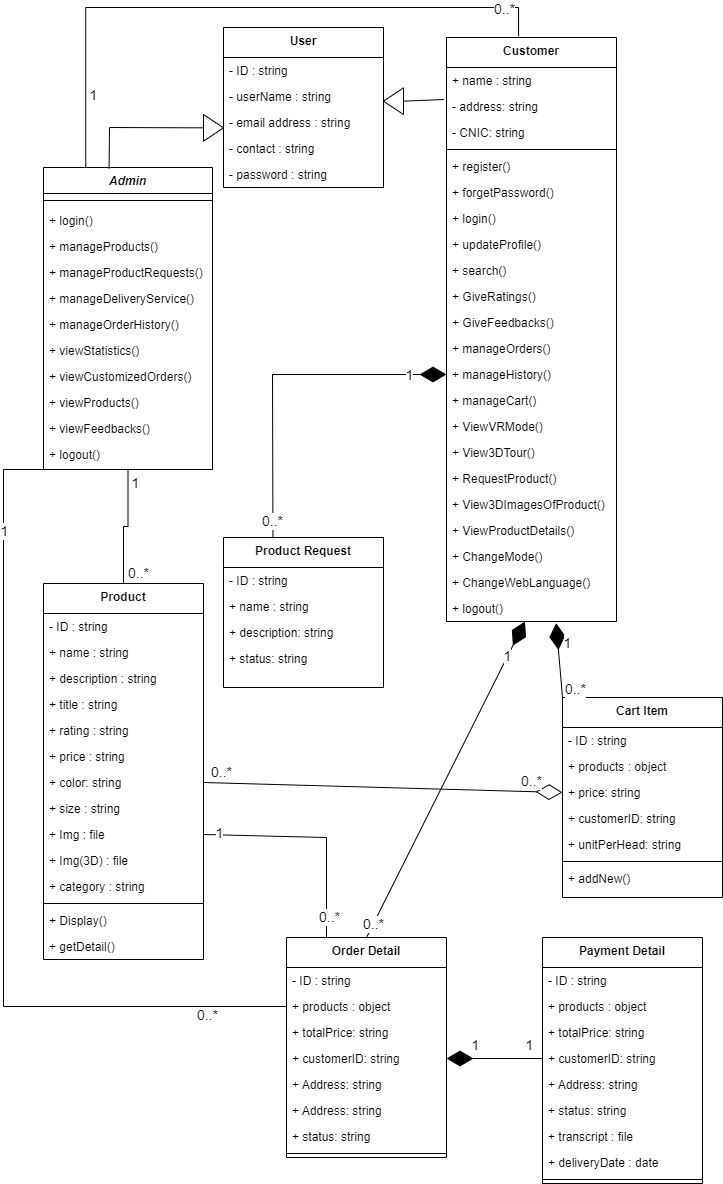
\includegraphics[width=15cm,height=15cm]{Diagrams/ClassDiagram.jpeg}
    \caption{System’s class diagram}
    \label{fig: System’s class diagram}
\end{figure}
\justifying
This class diagram represents the structure of our system. Classes, attributes of those classes, and relationships between classes are shown diagrammatically. Classes are represented by boxes for example user, and customer. Similarly, attributes of a class have been written inside the class box such as the id, username, and email of the class user. Relationships between classes have been represented by arrows between classes. Some arrows represent aggregation/composition.
\section{Entity Relationship Diagram}
\begin{figure}[H]
    \centering
    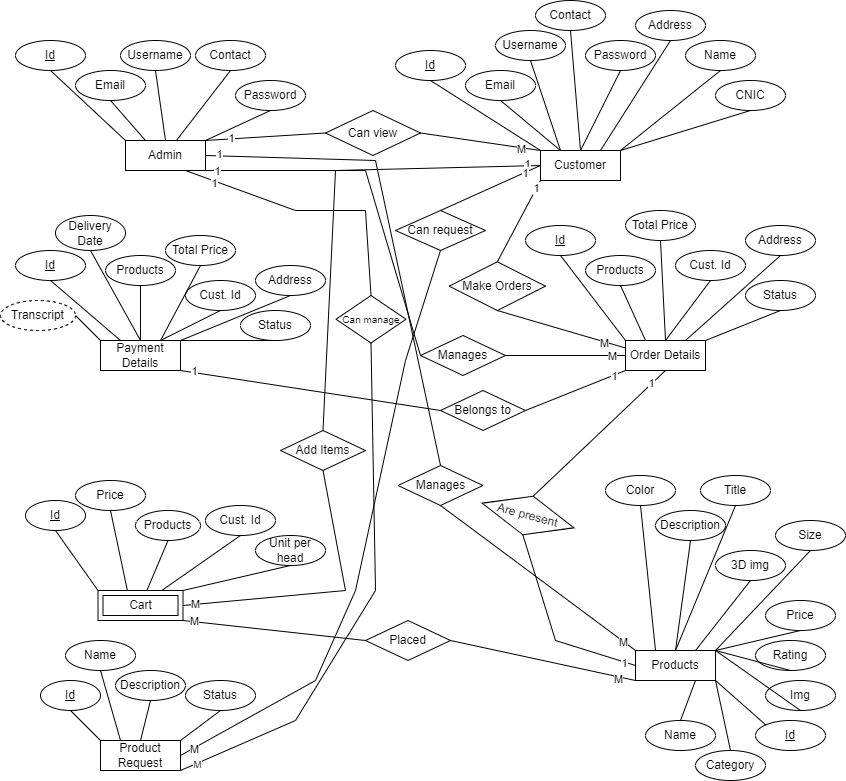
\includegraphics[width=14cm,height=15cm]{Diagrams/erDiagram.jpeg}
    \caption{System’s ERD(Entity Relationship Diagram)}
    \label{fig:System’s ERD(Entity Relationship Diagram)}
   
    \end{figure}
    \justifying
    This class diagram also represents the structure of the system. ERD diagram contains some symbols like rectangles, oval shapes, and lines. Rectangles represent entities which are customer, admin, payment details, cart e.t.c. Oval shapes are attributes of that entity. Similarly, the relationship between two entities is represented by a diamond in an arrow. And types of relationships such as one-to-one, one-to-many, and many-to-many are represented by small numbers near connecting points of the arrow. 


\section{Sequence Diagram}
Following are the sequence diagrams of the customer and admin of the web application that show the control structures between objects.
\subsection{Sequence Diagram for Admin}
\begin{figure}[H]
    \centering
    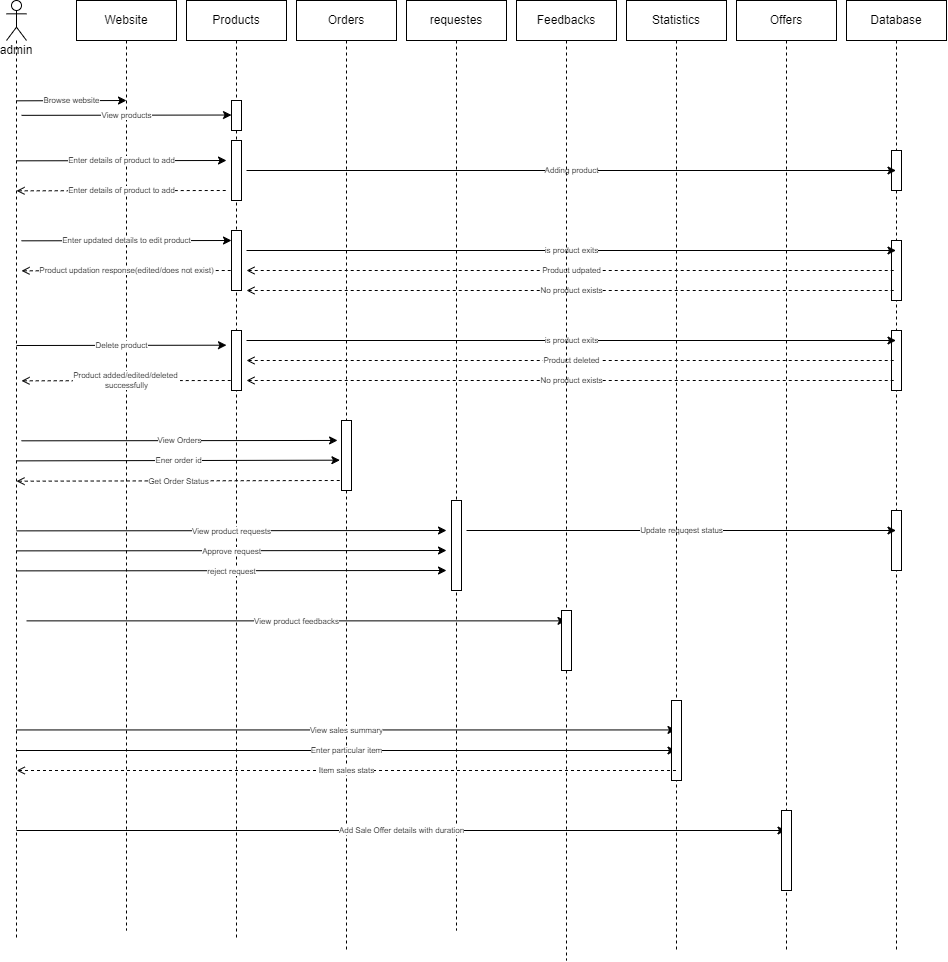
\includegraphics[width=14cm,height=15cm]{Diagrams/Admin_SequenceDiagram.png}
    \caption{System’s Sequence Diagram (Admin)}
    \label{fig: System’s Sequence Diagram (Admin)}

\end{figure}
\justifying
 This diagram shows the whole sequence of steps required by the admin to accomplish different tasks. For example view products, add products, view product requests, give responses to those requests e.t.c. In the diagram rectangles can be seen, these rectangles are modules of the system e.g products, orders, requests, feedback, e.t.c. Where the long bar under every module represents the lifetime for which the user would be interacting with that module. Arrows from user entities to different bars show the user’s purpose of interaction with that module. For example, the admin would interact with the product module to view the product shown in the diagram.
\subsection{Sequence Diagram for Customer}
\begin{figure}[H]
    \centering
    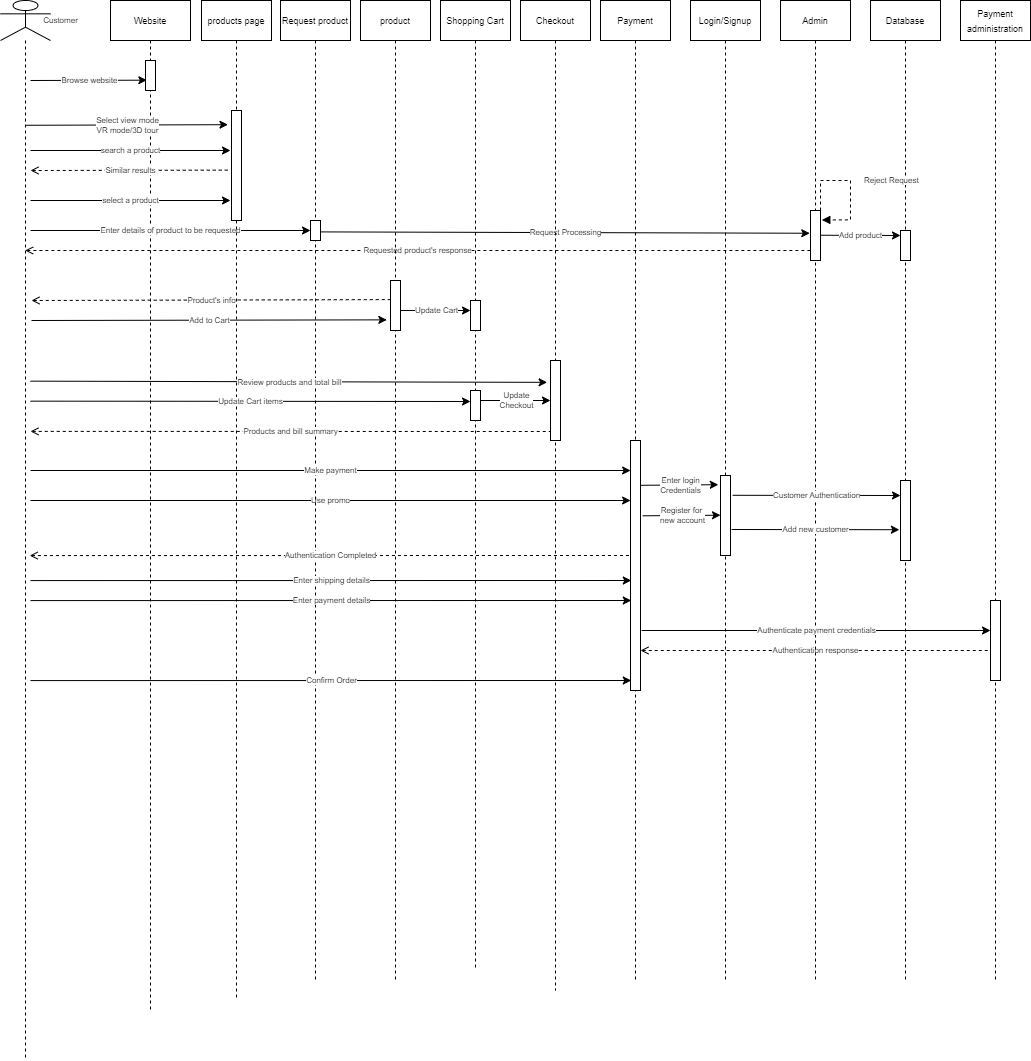
\includegraphics[width=14cm,height=15cm]{Diagrams/Customer_SequenceDiagram.png}
    \caption{System’s Sequence Diagram (Customer)}
    \label{fig: System’s Sequence Diagram (Customer)}
\end{figure}
\justifying
This diagram shows the whole sequence of steps required by customers to accomplish different tasks. For example viewing products, taking orders, making product requests, giving feedback to products e.t.c. In the diagram rectangles can be seen, these rectangles are modules of the system e.g products, shopping cart, payment, e.t.c. Where the long bar under every module represents the lifetime for which the user would be  interacting with that module. Arrows from the user entity to different bars show the user’s purpose of interaction with that module. For example, customers would interact with the product module to view the product shown in the diagram.